\documentclass[11pt,a4paper]{article}

\usepackage[czech]{babel}
\usepackage[utf8]{inputenc}
\usepackage{url}
\usepackage[textwidth=15.2cm,textheight=23cm]{geometry}
\usepackage{xcolor}
\usepackage{color}
\usepackage[unicode, colorlinks,hyperindex,plainpages=false,pdftex]{hyperref}
\usepackage{graphicx}
\usepackage{float}
\usepackage{multirow}
\usepackage[IL2]{fontenc}
\usepackage{siunitx}
\usepackage[bf]{caption}

\pdfcompresslevel=9

\newcommand{\myincludegraphics}[4]{
  \begin{figure}[!h]
  \centering
  \includegraphics[#1]{#2}
  \caption{#3.} \label{#4}
  \end{figure}
}

% titulní stránka a obsah
\newcommand{\titlepageandcontents}{
  % credits for template go to: Martin Striz
\begin{titlepage}

\vspace*{1cm}

\begin{figure}
  \centering
  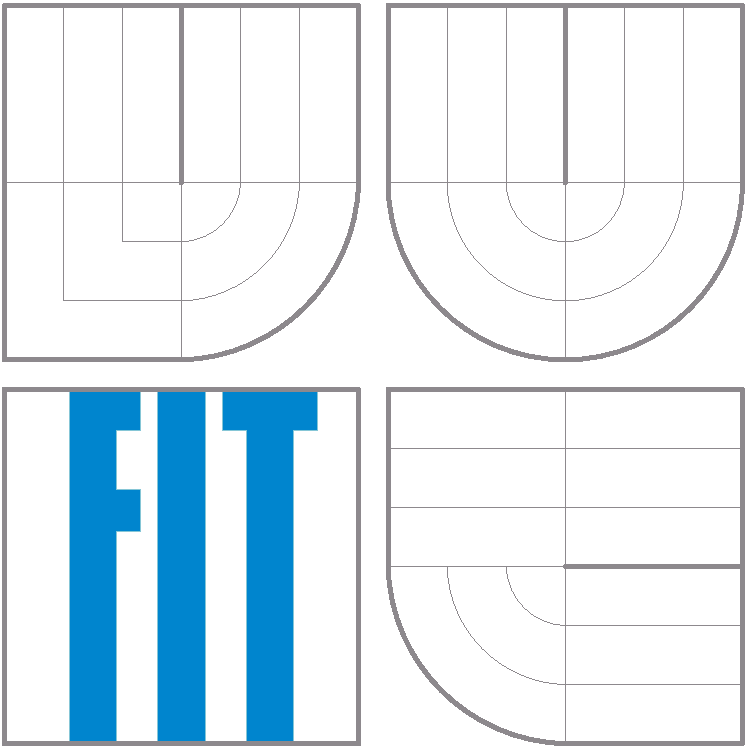
\includegraphics[height=6cm]{images/fit.pdf}
\end{figure}

\vspace*{5mm}

\begin{center}
\begin{Large}
Projekt do předmětu FYO -- Fyzikální optika
\end{Large}
\end{center}

\vspace*{5mm}

\begin{center}
\begin{Huge}
Fourierovská optika. Úprava obrazu.\\
\end{Huge}
\end{center}

\vspace*{1cm}

\begin{center}
\begin{Large}
\today
\end{Large}
\end{center}

\vfill

\begin{flushleft}
\begin{large}
\begin{tabular}{ll}

\bf Řešitel:\hspace{3mm} 
& Jan Wozniak (\verb_xwozni00@stud.fit.vutbr.cz_) \\
& Fakulta Informačních Technologií \\
& Vysoké Učení Technické v~Brně

\end{tabular}
\end{large}
\end{flushleft}

\end{titlepage}

% vim:set ft=tex expandtab enc=utf8:


  \pagestyle{plain}
  \pagenumbering{roman}
  \setcounter{page}{1}
  %\tableofcontents

  \newpage
  \pagestyle{plain}
  \pagenumbering{arabic}
  \setcounter{page}{1}
}









\begin{document}
\titlepageandcontents
\section{Úvod}
Obraz, jak jej vnímáme, může být reprezentován jako diskrétní dvourozměrná funkce $f[i,j]$.
Pro zobrazení v počítači lze rovněž pochopit tuto funkci jako matici, kde hodnoty $i$ a $j$ 
označují index řádku, resp. sloupce, této matice a hodnota prvku matice charakterizuje míru jasu pro daný
prvek matice -- pixel. V připadě, že se jedná o černobílý obrázek, jas je tvořen skalární hodnotou, 
velmi často 8 bitové hloubky, barevné hodnoty jsou reprezentovány pomocí složených datových typů
v konkrétním barevném modelu, tuto strukturu lze chápat jako vektorovou hodnotu. 

Existuje mnoho způsobů jak se zabývat optikou, optickým zobrazováním a úpravami obrazu.
Jeden z moderních pohledů spočívá ve využití Fourierovy transformace, která slouží k převodu
obrazu z prostorové domény do domény frekvenční. Této konverze lze docílit jak digitálně
díky matematickým vztahům ale analogickými postupy i s využitím fyzikálních zákonů a čočky.

\subsection{Historie}
Jean Baptiste Joseph Fourier objevil, že libovolná funkce může být rozložena v řadu 
harmonických funkcí o různých frekvencích a komplexních amplitudách, což se považuje za základ 
pro Fourierovskou optiku a harmonickou analýzu signálů.

Velmi přinosná pro aplikaci Fourierovy transformace byla práce pánů J. W. Cooleye a J. W. Tukeye,
kteří publikovali výrazné zefektivnění výpočtu diskrétní transformace zvané rychlá Fourierova
transformace. Tento algoritmus je dodnes nejpoužívanější variantou výpočtu transformace.

\section{Fyzikální princip}
Fourierovská optika popisuje šíření světla pomocí Fourierovy analýzy. Velmi zjednodušené vysvětlení by
se dalo definovat tak, že libovolnou vlnu ve volném prostoru je možně chápat jako superpozici rovinných 
vln. To znamená, je-li libovolná monochromatická 
vlna o vlnové délce $\lambda$ a komplexní amplitudě dané funkcí $f(x,y)$ složena z harmonických 
složek, pak každá harmonická složka odpovídá rovinné vlně. Každá rovinná vlna se šíří pod úhly 
$\theta x = sin^{-1}(\lambda v_x)$, $\theta y = sin^{-1}(\lambda v_y)$ a odpovídá složce s prostorovými 
frekvencemi $v_x$, $v_y$  a její amplituda je $F(v_x, v_y)$ což je Fourierova transformace funkce
$f(x,y)$. 

S využitím čočky, která zaostří rovinné vlny sdružené s harmonickýmí Fourierovými komponentami
vstupní funkce $f(x,y)$ do bodů $(\lambda v_x, \lambda v_y)$ v ohniskové rovině, můžeme jednotlivé
komponenty světla zpracovávat individuálně. To znamená, že rozložení světla v zadní ohniskové 
rovině čočky je úměrné Fourierově transformaci rozložení světla v přední ohniskové rovině \cite{dipl1}.

Demonstraci Fourierovy transformace v optice je možné fyzikálně provést pomocí difrakce. Na základě
Fresnelovy difrakce jsme teoreticky schopni dojít až k Fourierove transformaci. Tato difrakce je totiž
charakteristická tim, že v různě vzdálených rovinách pozorování lze sledovat různé difrakční obrazce. V jednom
teoretickém případu, je-li vzdálenost mezi objektem a stínítkem nekonečná, je vzniklý Fresnelův difrakční 
obrazec totožný s Fraunhoferovým difrakčním obrazcem daného objektu. S použitím optických pomůcek
jsme schopni vytvořit Fraunhoferův difrakční i v reálnějším schématu než-li v nekonečné vzdálenosti.

\subsection{Fraunhoferova difrakce}
Fraunhoferovu difrakci prakticky nemůžeme sledovat bez použití optiky (např. spojné čočky), proto není tolik
názorná jako Fresnelova difrakce. Poskytuje nám však informace o úhlovém rozložení difraktované intenzity 
(rovina pozorování Fraunhoferovy difrakce je v nekonečnu a jednotlivým bodům roviny v nekonečnu odpovídají směry). 
Vyjdeme-li z paprskové optiky, víme, že směrům v předmětovém prostoru odpovídají obrazové 
body v ohniskové rovině čočky. Z toho tedy vyplývá, že můžeme Fraunhoferovu difrakci pozorovat, 
vložíme-li za difraktující objekt čočku. Je ovšem třeba, aby na překážku dopadal rovnoběžný svazek světla \cite{difrakce}.

\begin{figure}[H]
\centering
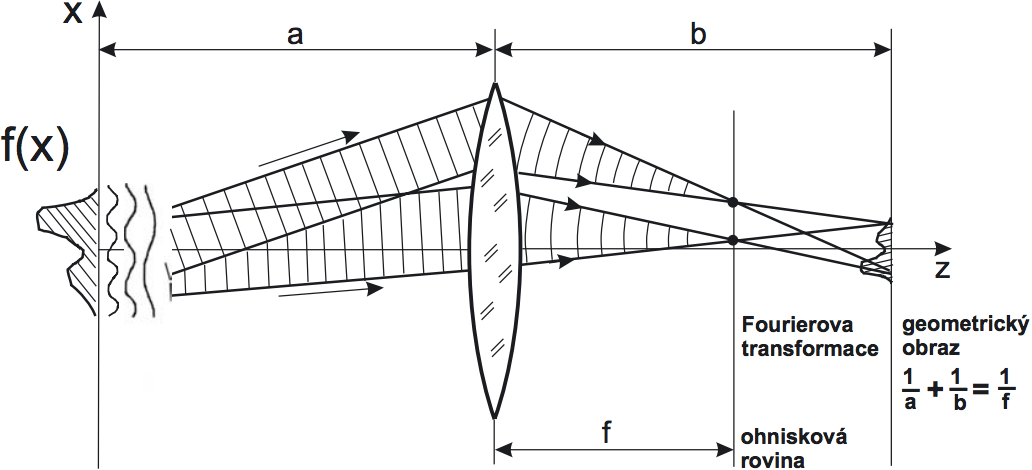
\includegraphics[width=14cm]{images/ft-cocka.png}
\caption{Optické zobrazování z hlediska Fourierovy transformace.}
\label{Fraunhofer}
\end{figure}

V levé části obrázku je zobrazovaný objekt, pomocí čočky je dosaženo zaostření paprsků a v ohniskové
rovině můžeme pozorovat obrazec Fourierovy transformace. Za Fourierovou rovinou se vytvoří obraz objektu. 
Franhoferova difrakce hraje zásadní úlohu právě v zobrazovacích soustavách. Každá taková soustava
se skládá ze dvou rovin

\begin{itemize}
\item \textbf{rovina s Franhouferovou difrakcí} -- primární obraz
\item \textbf{rovina obrazová} -- sekundární obraz
\end{itemize} 

K popisu sekundárního obrazu, Fraunhoferova obrazce a jejich vzájemného vztahu se používá tzv. 
Fourierova analýza a matematický aparát nazývaný Fourierovou transformací. 
Stejně jako je možné z obrazu získat pomocí Fourierovy transformace spektrum a ze spektra poté
inverzní Fourierovou transformací opět obraz věrný předloze, je možno zpětně převézt z Fraunhoferova 
difrakčního obrazce opět na obraz.
Zásahem do tohoto Fraunhoferova difrakčního obrazce (např. zacloněním 
některých jeho částí) lze potom snadno ovlivnit výsledný sekundární obraz. Tento se pak může 
velmi výrazně lišit od věrného obrazové předlohy -- objektu. 

\subsection{Prostorový filtr}
Ve své podstatě se jedná o optickou soustavu sestávající se ze dvou čoček se společným ohniskem.
Do roviny ohniska je umístěn filtr, prakticky se jedná o clonku na určité části Fourierova obrazu.
Svazek paprsků je zaostřen první čočkou, část je zacloněna filtrem, a druhou čočkou je opět přeměněn
na rovnoběžný svazek paprsků \cite{prost-filt}.
Filtr slouží k odstranění vad v obraze. Jde o difrakční a interferenční jevy,
které zapříčiňují lokální změny intenzity svazku. Tyto jevy mohou vznikat na pevných
částečkách ulpěných na povrchu optických prvků, bublinkách a mechanických poruchách ve skle
atd. Pro odstranění poruch způsobených těmito jevy lze použít filtr zvaný dolní propust. Ve frekvenční oblasti
jej lze realizovat jako malý otvor uprostřed obrazce. 
Velikosti dírkových clon se pohybují v řádech desítek $\si{\micro} m$ a jejich nejvhodnější
kombinace s určitým objektivem resp. mikroobjektivem je dána víceméně experimentálně. Je-li
clonka příliš malá, nelze se zbavit soustavy interferenčních proužků kolem stopy a je-li clonka
příliš velká, bude filtrace neúčinná.

Na obrázku \ref{dft} je schéma, jak taková optická soustava může být realizována pomocí 4-f systému,
což není nic jiného, než dvoučočkový zobrazovací systém. Skládá se ze tří podcelků:

\begin{itemize}
\item vstupní obrazec - čočka - Fourierova rovina
\item clona (stínítko)
\item Fourierova rovina - čočka - výstupní obrazec 
\end{itemize}

V první části dochází k rozkladu rovnoběžného svazku pomocí čočky, tento obraz je pomocí
clony filtrován, neboť jednotlivé složky jsou oddělené a každému bodu odpovídá právě jedna příslušná
prostorová frekvence. Filtrací jsme schopni selektivně ovlivnit, které frekvence propustíme a které
budeme blokovat. V poslední třetí části docházi k inverzní transformaci kde výsledkem je
odpovídajícím způsobem filtrovaný obraz. Kdyby do systému nebylo zahrnuto stínítko, výsledný
obraz je totožný se vstuním obrazem.

\begin{figure}[H]
\centering
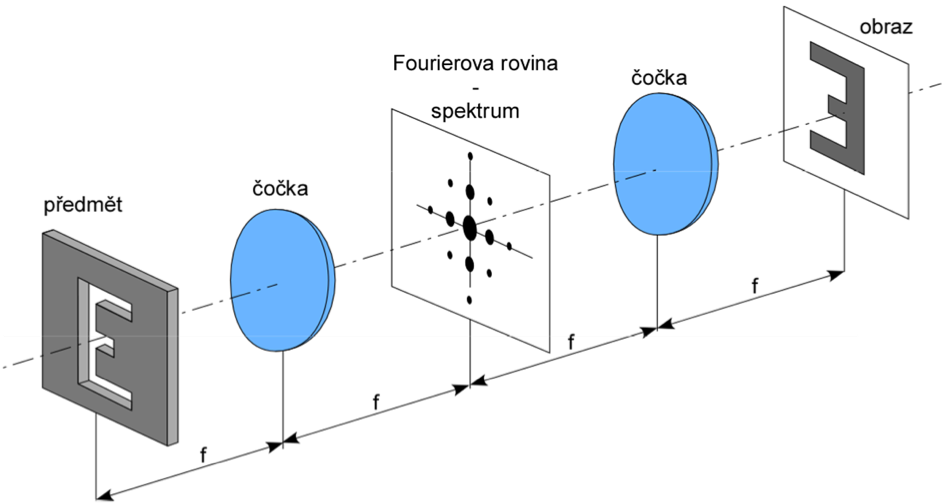
\includegraphics[width=14cm]{images/dft.png}
\caption{Prostorová filtrace.} %\cite{lib-prost}.}
\label{dft}
\end{figure}






\section{Matematické principy}
Tento projekt se zabývá úpravami obrazu, a jak bylo řečeno v úvodu, obraz lze pochopit jako 2D diskrétní 
signál, proto vztahy pro Fourierovu transformaci budou popsány rovněž z pohledu dvourozměrného signálu \cite{zre}.

\begin{equation}
F[k,l] = \sum_{m=0}^{N}{\sum_{n=0}^{N}{f[m,n]e^{(-i)\frac{2\pi km}{N}}\cdot e^{(-i)\frac{2\pi ln}{N}}}}
\label{dft}
\end{equation}

Kde $N$ jsou rozměry obrazu v pixelech, tedy $N^2$ dává celkový počet pixelů, a hodnoty $k$ a $l$ 
jsou diskrétní pozice v obrazu. Fourierova transformace pracuje s hodnotami intenzit vstupního obrazu
proto je nutné v případě barevného obrázku převézt z barevného modelu do hodnot odstínu šedé. Experimentálně
stanovena byla pro převod z RGB modelu rovnice~\ref{rgb}

\begin{equation}
Y = 0.299*R + 0.587*G + 0.114*B
\label{rgb}
\end{equation}

Převod se počítá pro každý pixel obrazu, kde $Y$ je výsledná jasová hodnota na dané pozici v obraze,
$R$, $G$ a $B$ jsou hodnoty intenzity v jednotlivých kanálech barevného modelu a konstanty násobící
kanálové složky jsou předem vhodně stanoveny aby odpovídaly skutečnému obrazovému vjemu.
Výsledkem Fourierovy transformace je obraz stejné velikosti jako byl vstupní, ale místo hodnoty jasu
je komplexní číslo.

Neboť velmi častou aplikací pro Fourierovu transformaci je prostorová filtrace, je vhodné uvést vztah 
pro konvoluci. Dále budou vztahy pro Fourierovu transformaci a konvoluci porovnávány z hlediska 
časové složitosti.
\begin{equation}
g[m,n] = \sum_{k=0}^{N}{\sum_{l=0}^{N}{f[k,l]\cdot h[m-k, n-l]}}
\label{konvoluce}
\end{equation}

\subsection{Spektrum}
Zobrazovaná funkce po provedení Fourierovy transformace se nazývá spektrum.  Toto spektrum má z hlediska 
definice Fourierovy transformace nejnižší frekvence v rozích obrazu. Je zvykem
pro názornější vizualizaci spektrum centrovat -- přesunout tak, aby nejnižší frekvence byly ve středu obrazu.
Díky symetrii spektra jej lze rozdělit na 4 kvadranty a ty pak podél příslušné diagonály prohodit. Počátek
funkce pak bude uprostřed obrazu.

\begin{figure}[H]
\centering
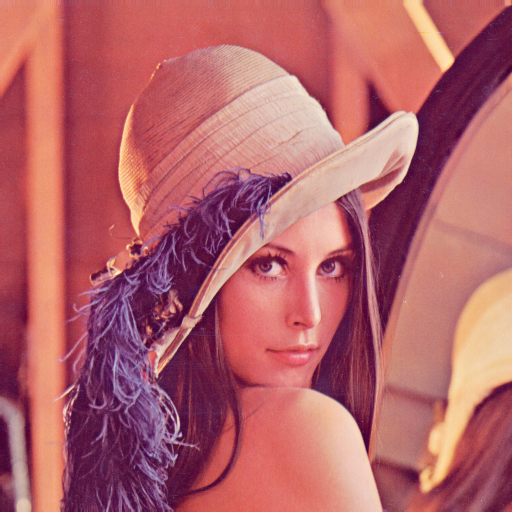
\includegraphics[width=7cm]{images/lena.png}
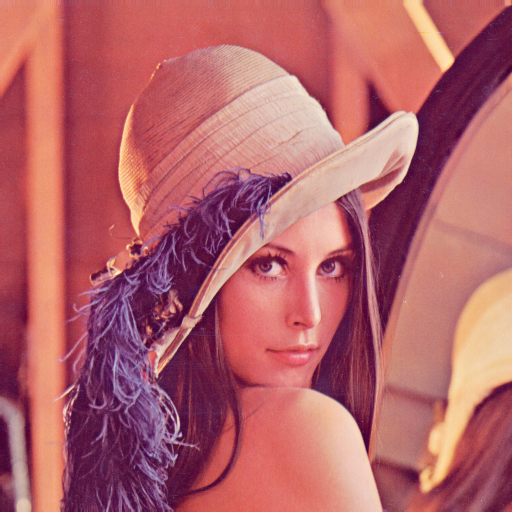
\includegraphics[width=7cm]{images/lena_spec.png}
\caption{Obraz a jeho centrované spektrum.}
\label{spec}
\end{figure}


\section{Aplikace}
Mimo zpracování obrazu je Fourierova transformace používaná v mnoha dalších oblastech jako například
řešení parciálních diferenciálních rovnic, rychlé násobení dvou velkých čísel. Výrazně lze pozorovat
důležitost Fourierovy transformace na faktu, že v dnešní době velká řada moderních DSP procesorů obsahuje
instrukce pro optimalizaci výpočtů rychlé Fourierovy transformace a zároveň existuje široké spektrum
paralelních implementací, urychlujících tento výpočet pomocí SIMD instrukční sady na běžných CPU \cite{xilinx}.

\subsection{Analýza složitosti}
Pro ideální využití Fourierovy transformace je vhodné znát i složitost výpočtu. Aby bylo  možné se
abstrahovat od konkrétní implementace či architektury stroje výpočet provádějící, 
pokusím se provést analýzu pouze na základě asymptotického časového chování algoritmu, paměťové
nároky nejsou vzhledem k charakteru výpočtu brány v úvahu.

Ze vzorce~\ref{dft} pro Fourierovu transformaci lze usoudit, že algoritmus ve dvou vnořených cyklech
násobí vektor $f[n,m]$ komplexní konstantou $e^{(-i)\frac{2\pi}{N}}$ umocněnou na $k\cdot m$ resp.
$l\cdot n$, z čehož by vyplýval horní odhad asymptotické složitosti $\mathcal{O}(N^3)$. 
Algoritmus výpočtu diskrétní Fourierovy transformace je možné výrazně urychlit metodou zvanou 
\textit{rychlá Fourierova transformace}. Její princip se zakládá na myšlence, že diskrétní fourierovu
transformaci délky N lze vyjádřit jako součet dvou transformací délky N/2, v jedné jsou liché a ve
druhé sudé vzorky a takto lze opět rekurzivně dělit obě poloviny. Výpočet rychlé Fourierovy transformace
spadá do nižší třídy složitosti $\mathcal{O}(N^2 \cdot \log_{2}{N})$. Jelikož aplikace filtru na signal ve
frekvenční doméně je realizovatelná s kvadratickou složitostí $\mathcal{O}(N^2)$, nejnáročnějším výpočtem
zůstává stále převod do frekvenční oblasti a zpět.

Výpočetní složitost konvoluce dvourozměrného signálu vzhledem k vzorci~\ref{konvoluce} je 
$\mathcal{O}(N^2 \cdot M^2)$, kde $N^2$ je velikost obrazu a $M^2$ je velikost konvolučního jádra. Je 
tedy patrné, že časová složitost aplikace filtru ve frekvenční oblasti spadá do nižší třídy složitosti 
oproti aplikaci filtru v prostorové oblasti. Zároveň jsme ale schopni usoudit, že máme-li dostatečně
malý obraz a filtr, reálná doba zpracování může být nižší pro výpočet pomocí konvoluce.

\subsection{Využití}
Fyzikální využití Franhouferovy difrakce je velmi široké, používá se například k analýze snímků z elektronového 
mikroskopu a snímků rozptylu částic (posouzení kvality zaostření, zjištění rozlišení, identifikace astigmatismu 
\dots), ke kontinuální kontrole tloušťky vláken a drátů a ke korekci zobrazovaní v optických soustavách. 

V oblasti počítačového vidění patří mezi jedny z nejpoužívanějších a nejrobustnějších obrazových příznaků 
Gaborův filter \cite{gabor}, který se skládá z banky několika Gáborových vlnek o různé magnitudě a orientaci, kde všechny
vlny lze generovat z bázové vlnky pomocí operací dilatace a rotace. Princip, jak tento filter funguje je velmi 
podobný principu, jakým analyzuje obraz lidský mozek. Pro popis Gáborovy vlnky je třeba vysvětlit termín
\textit{krátkodobá Fourierova transformace}, což je postupná aplikace Fourierovy transformace na krátké
úseky signálu. Tím získáme nejen možnost frekvenčně analyzovat signál ale zárověň zachováme informaci i 
z prostorové domény, bez které by přesná lokalizace objektů v obraze byla takřka nemožná. Těmto krátkým
úsekům se říká okna. Pokud aplikujeme Gaussovu funkci na tyto krátké okna, jedná se o speciální případ
krátkodobé Fourierovy transformace zvaný Gáborova vlnka.

Příbuzné transformace nalezly praktického využití i přímo v populárních datových formátech jako například
cosinova transformace, která tvoří základ pro kopresi obrazových dat ve formátu JPEG nebo diskrétní vlnková 
transformace pro bezztrátový formát PNG \cite{jpeg, png}.

\section{Závěr}
Výsledkem tohoto projektu bylo seznámit se se základy Fourierovské optiky a vytvořit vhodnou demonstrační
aplikaci na toto téma. Výstup aplikace je vidět i na obrázku \ref{spec}, je volně k dispozici včetně zdrojových
kódů ve veřejném git repozitáři \url{https://github.com/wozniakjan/FYO.git}.

\newpage

\bibliography{literatura} % viz. literatura.bib
\bibliographystyle{ieeetr}
\end{document}
